\documentclass[bigger]{beamer}

\usepackage{booktabs}
\usetheme{metropolis}
\metroset{block=fill}
\setbeamercolor{background canvas}{bg=white}
\usepackage[english]{babel}
\usepackage[utf8]{inputenc}

\title{Validity and Reliability of Student Models for Problem-Solving Activities}

\author{Tom\'a\v{s} Effenberger, Radek Pel\'anek\\[5mm]
%Masaryk University Brno\\
%Czech Republic

\includegraphics[width=.35\linewidth]{figures/al-logo}\\[3mm]
}

\newcommand{\img}[2]{
  \begin{center}
    \includegraphics[width=#1\linewidth]{figures/#2}
  \end{center}
}

\newcommand{\mute}[1]{
  {\color{gray}{#1}}
}


\date{LAK 2021}

\begin{document}

\frame{\titlepage}


\begin{frame}
  \frametitle{Overview}

  Context:\\student models for problem-solving activities
  \bigskip
  \pause

  Evaluation:\\
  next answer correctness: prevalent $\times$ insufficient
  \bigskip
  \pause

  Construction:\\
  answer correctness: prevalent $\times$ insufficient
\end{frame}


\begin{frame}
  \frametitle{Scenario}
  learning system for introductory programming\\
  several exercises (each with dozens of problems):
  \img{1.0}{exercises}
\end{frame}


\begin{frame}
  \frametitle{What we need a student model for?}
  \begin{enumerate}
    \item order problems
    \item order students
    \item performance predictions
  \end{enumerate}
\end{frame}


\begin{frame}
  \frametitle{Student model with performance measure}
  \hspace*{-0.9cm}
  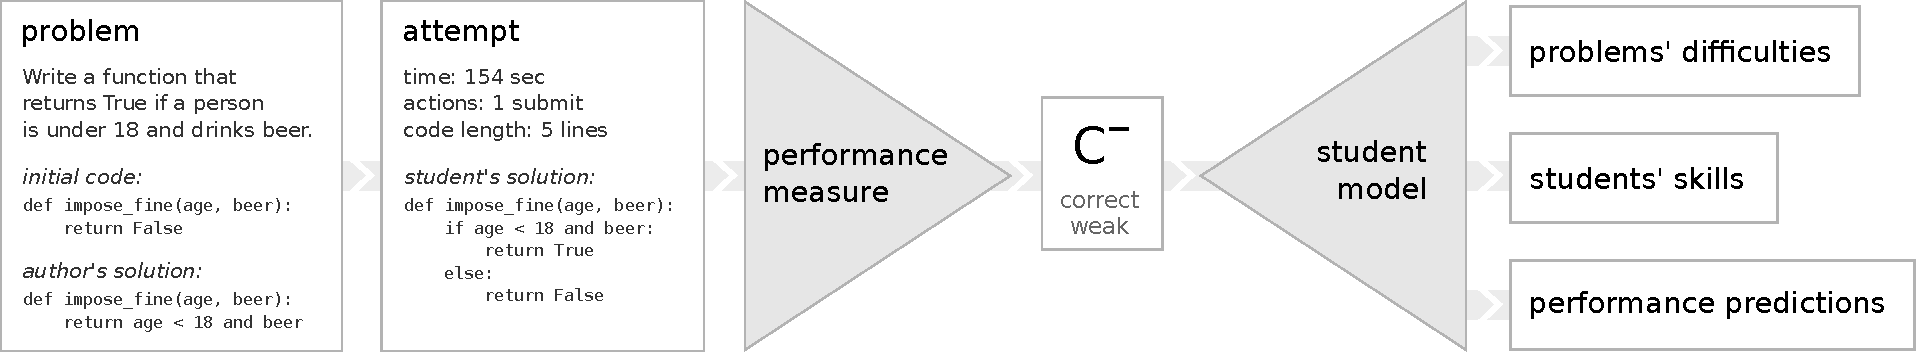
\includegraphics[width=1.15\linewidth]{figures/pipeline}
\end{frame}

\begin{frame}
  \frametitle{Typical evaluation}
  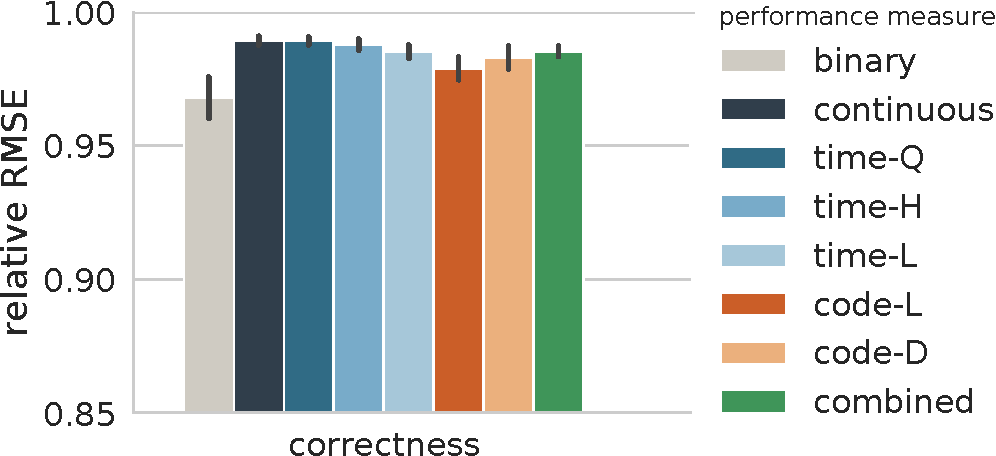
\includegraphics[height=3.5cm]{figures/next-answer-correctness}

  %\bigskip
  %\mute{\scriptsize
  %  Effenberger \& Pelánek. Impact of Methodological Choices on the Evaluation
  %  of Student Models. AIED 2020.
  %\par  % needed for correct line spacing
  %}

  \bigskip
  How would you interpret the results?
\end{frame}


\begin{frame}
  \frametitle{Less narrow picture}
  \hspace*{-0.65cm}
  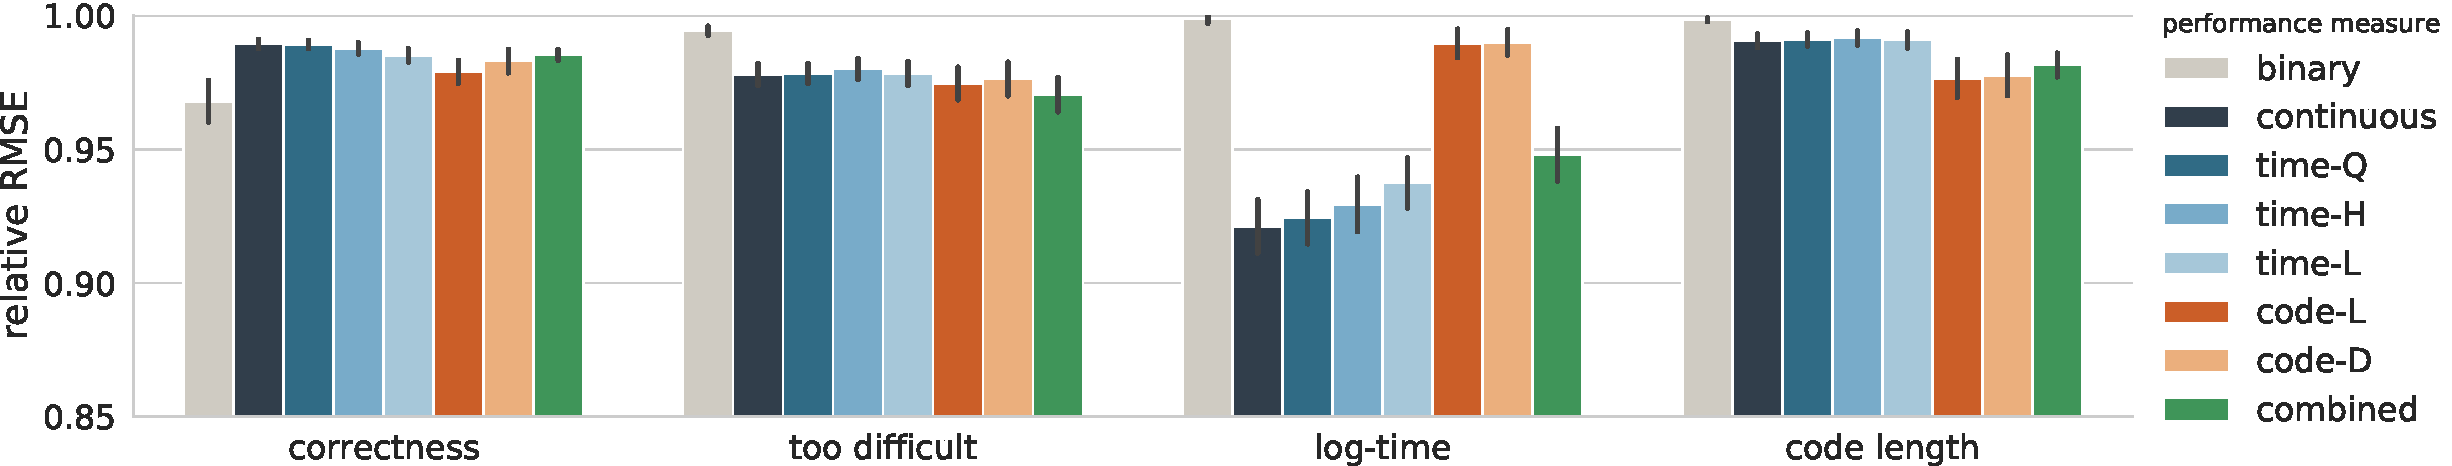
\includegraphics[width=1.1\linewidth]{figures/predictive-validity}
\end{frame}


\begin{frame}
  \frametitle{What do we really want?}
  valid model $\sim$ useful for the intended purposes
  \pause

  \medskip
  indirect evidence:
  \vspace{-0.1cm}
  \begin{itemize}
    \item criterion validity
    \begin{itemize}
      \item convergent
      \item predictive
      \begin{itemize}
        \item \alert{next answer correctness}
        \item next answer response time
        \item \ldots
      \end{itemize}
    \end{itemize}
    \item content validity
    %\item alignment with thought processes
    \item reliability
    \item \ldots
  \end{itemize}
\end{frame}


\begin{frame}
  \frametitle{Convergent validity}
  \bigskip
  \img{0.5}{convergent-validity}
  skill estimate based on correctness -- low correlation with\\
  skill estimate based on time/quality
\end{frame}


\begin{frame}
  \frametitle{Reliability}
  \begin{itemize}
    \item reliability $\sim$ consistency of the measurements
  \end{itemize}
  TODO: reliability vs validity visualization? (targets)
\end{frame}


\begin{frame}
  \frametitle{Split-half reliability of difficulties}
  \bigskip
  \img{0.9}{reliability-difficulties}
\end{frame}


\begin{frame}
  \frametitle{Odd-even reliability of skills}
  \bigskip
  \img{0.9}{reliability-skills}
\end{frame}


\begin{frame}
\frametitle{Message}
\begin{enumerate}
\item Next answer correctness is insufficient to validate student models.
\item Answer correctness is insufficient to model students in problem-solving activities.
\end{enumerate}
\end{frame}

\end{document}
